\documentclass[12pt]{article}

%% ── Page geometry ──────────────────────────────────────────────────────────
\usepackage[top=1.1in, bottom=1.1in, left=1.25in, right=1.25in]{geometry}

%% ── Core typography ────────────────────────────────────────────────────────
\usepackage[T1]{fontenc}
\usepackage[utf8]{inputenc}
\usepackage{mathptmx}          % Times New Roman body + math
\usepackage[scaled=0.92]{helvet}
\usepackage{microtype}         % Improved justification / protrusion
\usepackage{setspace}
\setstretch{1.15}

%% ── Mathematics ────────────────────────────────────────────────────────────
\usepackage{amsmath}
\usepackage{amssymb}
\usepackage{amsthm}
\usepackage{bm}

%% ── Tables ─────────────────────────────────────────────────────────────────
\usepackage{booktabs}
\usepackage{multirow}
\usepackage{makecell}
\usepackage{array}
\usepackage{tabularx}
\usepackage[table]{xcolor}
\definecolor{rowgray}{gray}{0.94}
\definecolor{headblue}{RGB}{220,230,245}
\definecolor{bestgreen}{RGB}{230,255,230}
\newcolumntype{C}[1]{>{\centering\arraybackslash}p{#1}}
\newcolumntype{L}[1]{>{\raggedright\arraybackslash}p{#1}}
\newcolumntype{R}[1]{>{\raggedleft\arraybackslash}p{#1}}

%% ── Figures ─────────────────────────────────────────────────────────────────
\usepackage{graphicx}
\usepackage{subcaption}
\graphicspath{{../figures/}}

%% ── References ──────────────────────────────────────────────────────────────
\usepackage[numbers,sort&compress]{natbib}
\bibliographystyle{plainnat}

%% ── Hyperlinks ───────────────────────────────────────────────────────────────
\usepackage[
  colorlinks=true,
  linkcolor=blue!60!black,
  citecolor=blue!60!black,
  urlcolor=blue!60!black,
  pdftitle={When Does Chain-of-Thought Hurt Reranking?},
  pdfauthor={Muhammad Raheel Anwar},
]{hyperref}
\usepackage{cleveref}

%% ── Algorithms ───────────────────────────────────────────────────────────────
\usepackage{algorithm}
\usepackage{algpseudocode}
\algrenewcommand\algorithmicindent{1.0em}

%% ── Code listings ────────────────────────────────────────────────────────────
\usepackage{listings}
\lstset{
  basicstyle=\footnotesize\ttfamily,
  backgroundcolor=\color{gray!8},
  frame=single,
  rulecolor=\color{gray!40},
  breaklines=true,
  numbers=left,
  numberstyle=\tiny\color{gray},
  xleftmargin=2em,
  framexleftmargin=1.5em,
  aboveskip=8pt,
  belowskip=4pt,
}

%% ── Misc ─────────────────────────────────────────────────────────────────────
\usepackage{enumitem}
\usepackage{parskip}
\setlength{\parskip}{4pt}
\usepackage{titlesec}
\titleformat{\section}{\large\bfseries}{\thesection.}{0.6em}{}
\titleformat{\subsection}{\normalsize\bfseries}{\thesubsection}{0.6em}{}
\titleformat{\subsubsection}{\normalsize\itshape\bfseries}{\thesubsubsection}{0.6em}{}
\usepackage{fancyhdr}
\pagestyle{fancy}
\fancyhf{}
\rhead{\small\textit{When Does Chain-of-Thought Hurt Reranking?}}
\lhead{\small\textit{M.\ R.\ Anwar}}
\cfoot{\thepage}
\renewcommand{\headrulewidth}{0.4pt}

%% ── Theorem environments ─────────────────────────────────────────────────────
\newtheorem{definition}{Definition}
\newtheorem{proposition}{Proposition}
\newtheorem{remark}{Remark}

%% ── Utility macros ───────────────────────────────────────────────────────────
\newcommand{\ndcg}{NDCG@10}
\newcommand{\direct}{\textsc{Direct-Point}}
\newcommand{\reason}{\textsc{Reason-Point}}
\newcommand{\router}{\textsc{Router}}
\newcommand{\CoT}{CoT}
\newcommand{\etal}{\textit{et al.}}
\newcommand{\eg}{\textit{e.g.}}
\newcommand{\ie}{\textit{i.e.}}
\newcommand{\cf}{\textit{cf.}}
\newcommand{\vs}{\textit{vs.}}
\DeclareMathOperator{\softmax}{softmax}

\begin{document}

%% ── Title block ──────────────────────────────────────────────────────────────
\begin{titlepage}
\centering
\vspace*{1.5cm}

{\LARGE\bfseries When Does Chain-of-Thought Hurt Reranking?\par}
\vspace{0.35em}
{\Large A Systematic Zero-Shot Analysis Across Query Complexity,\\[0.2em]
Reasoning Length, and Selective Routing\par}

\vspace{1.8cm}

{\large Muhammad Raheel Anwar\par}
\vspace{0.3em}
{\normalsize National University of Sciences \& Technology (NUST)\par}
\vspace{0.2em}
{\small \texttt{mranwar.mscs22seecs@seecs.edu.pk}\par}

\vspace{1.8cm}

{\small\itshape Submitted as a preprint.\par}

\vspace{2cm}

\begin{abstract}
\noindent
Chain-of-thought (\CoT{}) prompting has demonstrated strong gains on multi-step
reasoning tasks, yet its utility in document reranking remains contested.
Supervised approaches report improvements from \CoT{}-augmented rerankers, while
concurrent negative results challenge whether reasoning is necessary at all.
Yet the zero-shot regime, where no labeled data or fine-tuning is
available, has not been systematically studied.

We present the first zero-shot analysis of \CoT{} in pointwise document
reranking.  Using Qwen2.5-3B-Instruct on five benchmarks (BEIR and BRIGHT), we
show that direct logit scoring (\direct{}) consistently outperforms
reason-then-score (\reason{}) across all datasets ($\Delta$\ndcg{} from
$0.001$ to $0.124$; mean $\Delta=0.048$).  Stratifying queries into complexity
terciles reveals that \CoT{} degrades performance uniformly across simple,
medium, and complex queries (Mann--Whitney $U$, all $p<0.05$).  A
complexity-aware router that directs complex queries to \CoT{} likewise fails
to recover baseline performance.  All experiments are reproducible on a single
free-tier Google Colab T4 GPU.
\end{abstract}

\vfill
\end{titlepage}

\tableofcontents
\newpage

%% ============================================================
\section{Introduction}
\label{sec:intro}
%% ============================================================

The rise of instruction-following large language models has fundamentally
transformed document reranking.  Where first-generation neural
rerankers such as monoBERT~\citep{nogueira2019passage} and
monoT5~\citep{nogueira2020document} relied on bidirectional encoders trained
specifically for relevance estimation, modern LLM-based rerankers use
generative models that can reason about relevance in natural language.
This shift has stimulated substantial interest in applying chain-of-thought
(\CoT{}) prompting~\citep{wei2022chain} to reranking: if a model can
\emph{explain} why a document is relevant before committing to a score,
the reasoning may discipline the score toward higher quality.

The intuition is particularly compelling for complex queries involving causal
reasoning, multi-hop inference, or domain-specific terminology.  Several
recently proposed systems have operationalized this idea through supervised
fine-tuning and reinforcement learning:
Rank1~\citep{weller2025rank1} leverages test-time compute;
Rank-R1~\citep{zhuang2025rankr1} applies NDCG-rewarded RL;
ReasonRank~\citep{liu2025reasonrank}, REARANK~\citep{zhang2025rearank},
and ReasoningRank~\citep{ji2024reasoningrank} introduce distillation- and
agent-based formulations; and Rank-K~\citep{yang2025rankk} extends the
paradigm to listwise reranking.

Yet the empirical record has grown increasingly equivocal.
Lu~\etal~\citep{lu2025rethinking} showed, through careful ablations, that
\CoT{} \emph{consistently degrades} pointwise reranking when applied via
fine-tuning on Qwen2.5-4B and Qwen2.5-8B.  Jedidi~\etal~\citep{jedidi2025dont}
independently demonstrated that reasoning is unnecessary for passage reranking,
and Fan~\etal~\citep{fan2025tfrank} proposed TFRank, a think-free approach
that matches or exceeds reasoning-based rerankers at a fraction of the cost.
These results collectively challenge the foundational assumption that
deliberation improves relevance judgment.

All prior negative results, however, concern the \emph{supervised}
setting.  The zero-shot regime, where the model receives no task-specific
training, remains unexplored.  This is not a narrow technical gap: the majority
of real-world LLM deployments operate zero-shot, where labeled relevance data is
unavailable or fine-tuning is infeasible.  Three related questions have received
no systematic treatment: (i) does \CoT{} harm persist uniformly across query
complexity, or does it become helpful for queries requiring multi-step inference?
(ii) within the \CoT{} condition, does reasoning-chain length predict ranking
quality? and (iii) can a simple complexity-aware routing heuristic recover
baseline performance without retraining?

\paragraph{Contributions.}
We address all three questions through a systematic zero-shot study.

\begin{enumerate}[leftmargin=2em, label=\textbf{C\arabic*.}]
  \item \textbf{Zero-shot confirmation at 3B scale.}  We demonstrate that
        \CoT{} degrades zero-shot pointwise reranking with a 3B
        instruction-tuned model across five heterogeneous benchmarks.
        \direct{} outperforms \reason{} on all five datasets (\ndcg{} gaps
        of $0.001$--$0.124$, mean $\Delta=0.048$).

  \item \textbf{Uniform complexity degradation.}  Query-length tercile
        stratification reveals statistically significant \CoT{} degradation
        across simple, medium, and complex queries ($p<0.05$, Mann--Whitney
        $U$ test), ruling out any complexity-conditional benefit.

  \item \textbf{Quantified length--quality relationship.}  Within the
        \reason{} condition, CoT chain length shows near-zero linear
        correlation with per-query \ndcg{} (Pearson $r=0.010$, $p=0.78$)
        and a weak positive monotonic trend (Spearman $\rho=0.14$,
        $p<0.0001$) that does not overcome the direct-scoring advantage.

  \item \textbf{Systematic negative routing result.}  A complexity-aware
        router that delegates complex queries to \reason{} underperforms the
        pure-\direct{} baseline on all five datasets.

  \item \textbf{Colab-reproducible baseline.}  All experiments run on a
        single free-tier Google Colab T4 GPU (15.6\,GB VRAM), requiring no
        proprietary data, fine-tuning, or specialized infrastructure.
\end{enumerate}

The remainder of this paper is organized as follows.
\Cref{sec:background} provides background on neural reranking, \CoT{}, and
logit-based scoring.  \Cref{sec:related} surveys related work.
\Cref{sec:method} formalizes the task and describes our methodology.
\Cref{sec:results} presents experimental results.  \Cref{sec:analysis}
offers interpretive discussion.  \Cref{sec:repro} details reproducibility.
\Cref{sec:conclusion} concludes.

%% ============================================================
\section{Background}
\label{sec:background}
%% ============================================================

\subsection{Neural Document Reranking}

The standard neural information retrieval pipeline is a two-stage cascade.
In the \emph{retrieval stage}, a fast approximate method, most commonly
BM25~\citep{robertson2009probabilistic}, produces a candidate set of the
top-$k$ documents for each query.  BM25 models relevance as a weighted
term-frequency--inverse-document-frequency score normalized by document
length, and remains competitive despite its purely lexical nature.  In the
\emph{reranking stage}, a more expressive model rescores the candidate set
and produces a refined ranking.

The reranking stage has evolved through several generations.  BERT-based
cross-encoders~\citep{nogueira2019passage} take the concatenated
query--document pair as input and output a relevance logit.
MonoT5~\citep{nogueira2020document} extended this to sequence-to-sequence
models, framing relevance as a conditional generation problem: the probability
assigned to the token ``true'' given the input serves as the relevance score.
This logit-based scoring paradigm directly informs our \direct{} baseline.
LLM-based rerankers have further advanced the state of the art, particularly
on out-of-domain and reasoning-intensive
benchmarks~\citep{sun2023chatgpt, pradeep2023rankvicuna, pradeep2023rankzephyr}.

\subsection{Chain-of-Thought Prompting}

\CoT{} prompting, introduced by Wei~\etal~\citep{wei2022chain}, elicits
intermediate reasoning steps from LLMs before producing a final answer,
demonstrating dramatic improvements on multi-step mathematical and commonsense
reasoning tasks.  Kojima~\etal~\citep{kojima2022large} showed that simply
appending ``Let's think step by step'' to a prompt suffices to elicit reasoning
without few-shot demonstrations.

\begin{definition}[Chain-of-Thought Prompting]
  Given an input $x$ and a model $\mathcal{M}$, chain-of-thought prompting
  solicits a sequence of intermediate reasoning tokens
  $r = (r_1, r_2, \ldots, r_T)$ prior to the final answer token $a$, such
  that $\mathcal{M}(a \mid x, r) > \mathcal{M}(a \mid x)$ in expected task
  performance.
\end{definition}

The conditions under which \CoT{} provides gains are not universal.  Several
studies have observed degradation when the required reasoning is shallow or
when the model already holds a strong prior over the answer~\citep{kadavath2022language}.
Document reranking may be one such task: relevance judgments are often
categorical and do not require the kind of multi-step derivation that \CoT{}
was designed to support.

\subsection{Pointwise Scoring via Token Logits}

The logit-based pointwise scoring approach converts a generative LLM into a
relevance scorer without any training.  Given query $q$ and document $d$, the
model is prompted to produce a binary judgment.  Rather than sampling the output,
we extract the \emph{logits} at the decision position and apply a two-class
softmax:

\begin{equation}
  s(q, d) = \frac{\exp\!\left(\ell_{\texttt{true}}\right)}
                 {\exp\!\left(\ell_{\texttt{true}}\right)
                  + \exp\!\left(\ell_{\texttt{false}}\right)}
  \label{eq:score}
\end{equation}

\noindent
where $\ell_{\texttt{true}}$ and $\ell_{\texttt{false}}$ are the unnormalized
logits for the target tokens at the decision position.  The two variants of our
study differ in \emph{where} this extraction occurs: at the end of the input
prompt (\direct{}) or after a generated reasoning chain (\reason{}).

\subsection{Evaluation Metric}

We report Normalized Discounted Cumulative Gain at rank 10 (\ndcg{}) as the
primary evaluation metric~\citep{jarvelin2002cumulated}.  For a ranking of
$n$ documents with graded relevance labels $\mathrm{rel}_i$:

\begin{equation}
  \mathrm{DCG}@10 = \sum_{i=1}^{10}
    \frac{2^{\mathrm{rel}_i} - 1}{\log_2(i+1)}, \qquad
  \mathrm{NDCG}@10 = \frac{\mathrm{DCG}@10}{\mathrm{IDCG}@10}
\end{equation}

\noindent
\ndcg{} is bounded in $[0,1]$ and weights relevant documents appearing earlier
in the ranking more heavily.  We prefer it over rank-biased
overlap~\citep{webber2010similarity} for comparability with the existing
reranking literature.

%% ============================================================
\section{Related Work}
\label{sec:related}
%% ============================================================

\subsection{LLM-Based Reranking}

The application of large language models to document reranking accelerated
substantially after Sun~\etal~\citep{sun2023chatgpt} demonstrated that
GPT-3.5-based RankGPT serves as a competitive listwise reranker without
task-specific training.  Pradeep~\etal{} extended this paradigm with
open-source alternatives, RankVicuna~\citep{pradeep2023rankvicuna} and
RankZephyr~\citep{pradeep2023rankzephyr}, showing that 7B-parameter models
can achieve competitive performance when appropriately prompted.  Pointwise
scoring methods remain attractive for their $O(k)$ complexity and natural
parallelizability over the candidate set.

\subsection{Reasoning-Enhanced Reranking}

The emergence of strong reasoning models such as
DeepSeek-R1~\citep{guo2025deepseekr1} motivated applying \CoT{} techniques
to reranking through supervised adaptation.
Rank1~\citep{weller2025rank1} augments pointwise reranking with test-time
compute via extended reasoning traces.  Rank-R1~\citep{zhuang2025rankr1}
applies RL with NDCG-based reward signals.
ReasonRank~\citep{liu2025reasonrank} and REARANK~\citep{zhang2025rearank}
propose agent-based and multi-stage formulations.
ReasoningRank~\citep{ji2024reasoningrank} uses knowledge distillation to
transfer reasoning capabilities to smaller student models.
Rank-K~\citep{yang2025rankk} extends the paradigm to listwise reranking.
What unites these approaches is their reliance on labeled data and specialized
training; none addresses the zero-shot regime.

\subsection{Negative Results and Efficiency-Motivated Approaches}

Lu~\etal~\citep{lu2025rethinking} provide the most comprehensive negative
result to date, showing through controlled ablations that \CoT{} consistently
degrades pointwise reranking across fine-tuned variants of Qwen2.5-4B and
Qwen2.5-8B.  Their analysis identifies reasoning-induced \emph{score
distortion} as the likely mechanism: deliberation perturbs the logit
distribution in ways that harm ranking calibration.  Jedidi~\etal~\citep{jedidi2025dont}
independently argue that passage reranking does not require the kind of
multi-step inference that \CoT{} was designed to elicit.
Fan~\etal~\citep{fan2025tfrank} propose TFRank, which explicitly bypasses
reasoning and achieves competitive or superior performance on both standard and
reasoning-intensive benchmarks.

\subsection{Query Complexity and Selective Retrieval}

Query performance prediction (QPP)~\citep{cronen2002predicting} estimates
retrieval system performance on a per-query basis, with query length and
clarity score among the oldest predictors.  Selective
retrieval~\citep{arabzadeh2021shallow} has shown that routing queries to
different strategies based on predicted difficulty can improve average
performance.  The BRIGHT benchmark~\citep{su2024bright} was specifically
designed to evaluate retrieval under reasoning-intensive queries, providing a
natural high-complexity counterpart to standard BEIR datasets.  To our
knowledge, no prior work has systematically measured the interaction between
query complexity and \CoT{} in reranking.

\subsection{Positioning This Work}

\Cref{tab:positioning} positions our paper relative to the most closely related
prior studies.

\begin{table}[htbp]
\caption{Positioning of this work relative to prior studies.  Columns indicate:
         zero-shot evaluation, query complexity stratification, reasoning-length
         analysis, and reproducibility on free compute.
         \checkmark~= yes; \texttimes~= no; --~= partial.}
\label{tab:positioning}
\centering
\small
\setlength{\tabcolsep}{7pt}
\renewcommand{\arraystretch}{1.25}
\begin{tabular}{@{}lcccc@{}}
\toprule
\textbf{Study} &
\makecell{\textbf{Zero-Shot}\\\textbf{Eval.}} &
\makecell{\textbf{Complexity}\\\textbf{Stratif.}} &
\makecell{\textbf{Length--Quality}\\\textbf{Analysis}} &
\makecell{\textbf{Free-Tier}\\\textbf{Reproducible}} \\
\midrule
Lu~\etal~\citep{lu2025rethinking}        & \texttimes & \texttimes & \texttimes & \texttimes \\
Jedidi~\etal~\citep{jedidi2025dont}      & --         & \texttimes & \texttimes & \texttimes \\
Fan~\etal~\citep{fan2025tfrank}          & \checkmark & \texttimes & \texttimes & \texttimes \\
Weller~\etal~\citep{weller2025rank1}     & \texttimes & \texttimes & \texttimes & \texttimes \\
Zhuang~\etal~\citep{zhuang2025rankr1}    & \texttimes & \texttimes & \texttimes & \texttimes \\
\textbf{This work}                       & \checkmark & \checkmark & \checkmark & \checkmark \\
\bottomrule
\end{tabular}
\end{table}

%% ============================================================
\section{Methodology}
\label{sec:method}
%% ============================================================

\subsection{Task Definition and Research Questions}

\begin{definition}[Pointwise Document Reranking]
  Given a query $q \in \mathcal{Q}$ and a candidate set
  $\mathcal{D}_q = \{d_1, d_2, \ldots, d_k\}$ produced by a first-stage
  retrieval system, the reranking task is to produce a permutation
  $\pi : [k] \to [k]$ such that documents with higher relevance to $q$ are
  assigned smaller ranks.  In the pointwise paradigm, this is accomplished by
  assigning a scalar score $s(q, d_i) \in [0, 1]$ to each candidate
  independently and sorting by score in descending order.
\end{definition}

We study the \emph{zero-shot} setting exclusively: the scoring function
$s(q,d)$ is instantiated by an instruction-tuned LLM with no task-specific
fine-tuning, and each document is scored independently.  Our four research
questions are:

\begin{description}[leftmargin=1em, labelindent=0.5em]
\item[\textbf{RQ1}:]
  Does \CoT{} improve or degrade zero-shot pointwise reranking quality
  compared to direct logit scoring?
\item[\textbf{RQ2}:]
  Is the \CoT{} effect moderated by query complexity? Specifically, does
  \CoT{} become beneficial for complex queries?
\item[\textbf{RQ3}:]
  Within the \CoT{} condition, is reasoning-chain length correlated with
  per-query ranking quality?
\item[\textbf{RQ4}:]
  Can a complexity-aware selective router recover the direct-scoring baseline
  without retraining?
\end{description}

\subsection{System Overview}

\Cref{fig:pipeline} illustrates the overall system architecture.  The pipeline
proceeds in three stages: (1)~BM25 first-stage retrieval producing $k=100$
candidates per query; (2)~zero-shot LLM reranking under either \direct{} or
\reason{}; and (3)~analysis comprising complexity stratification,
CoT-length measurement, and selective routing evaluation.

\begin{figure}[htbp]
\centering
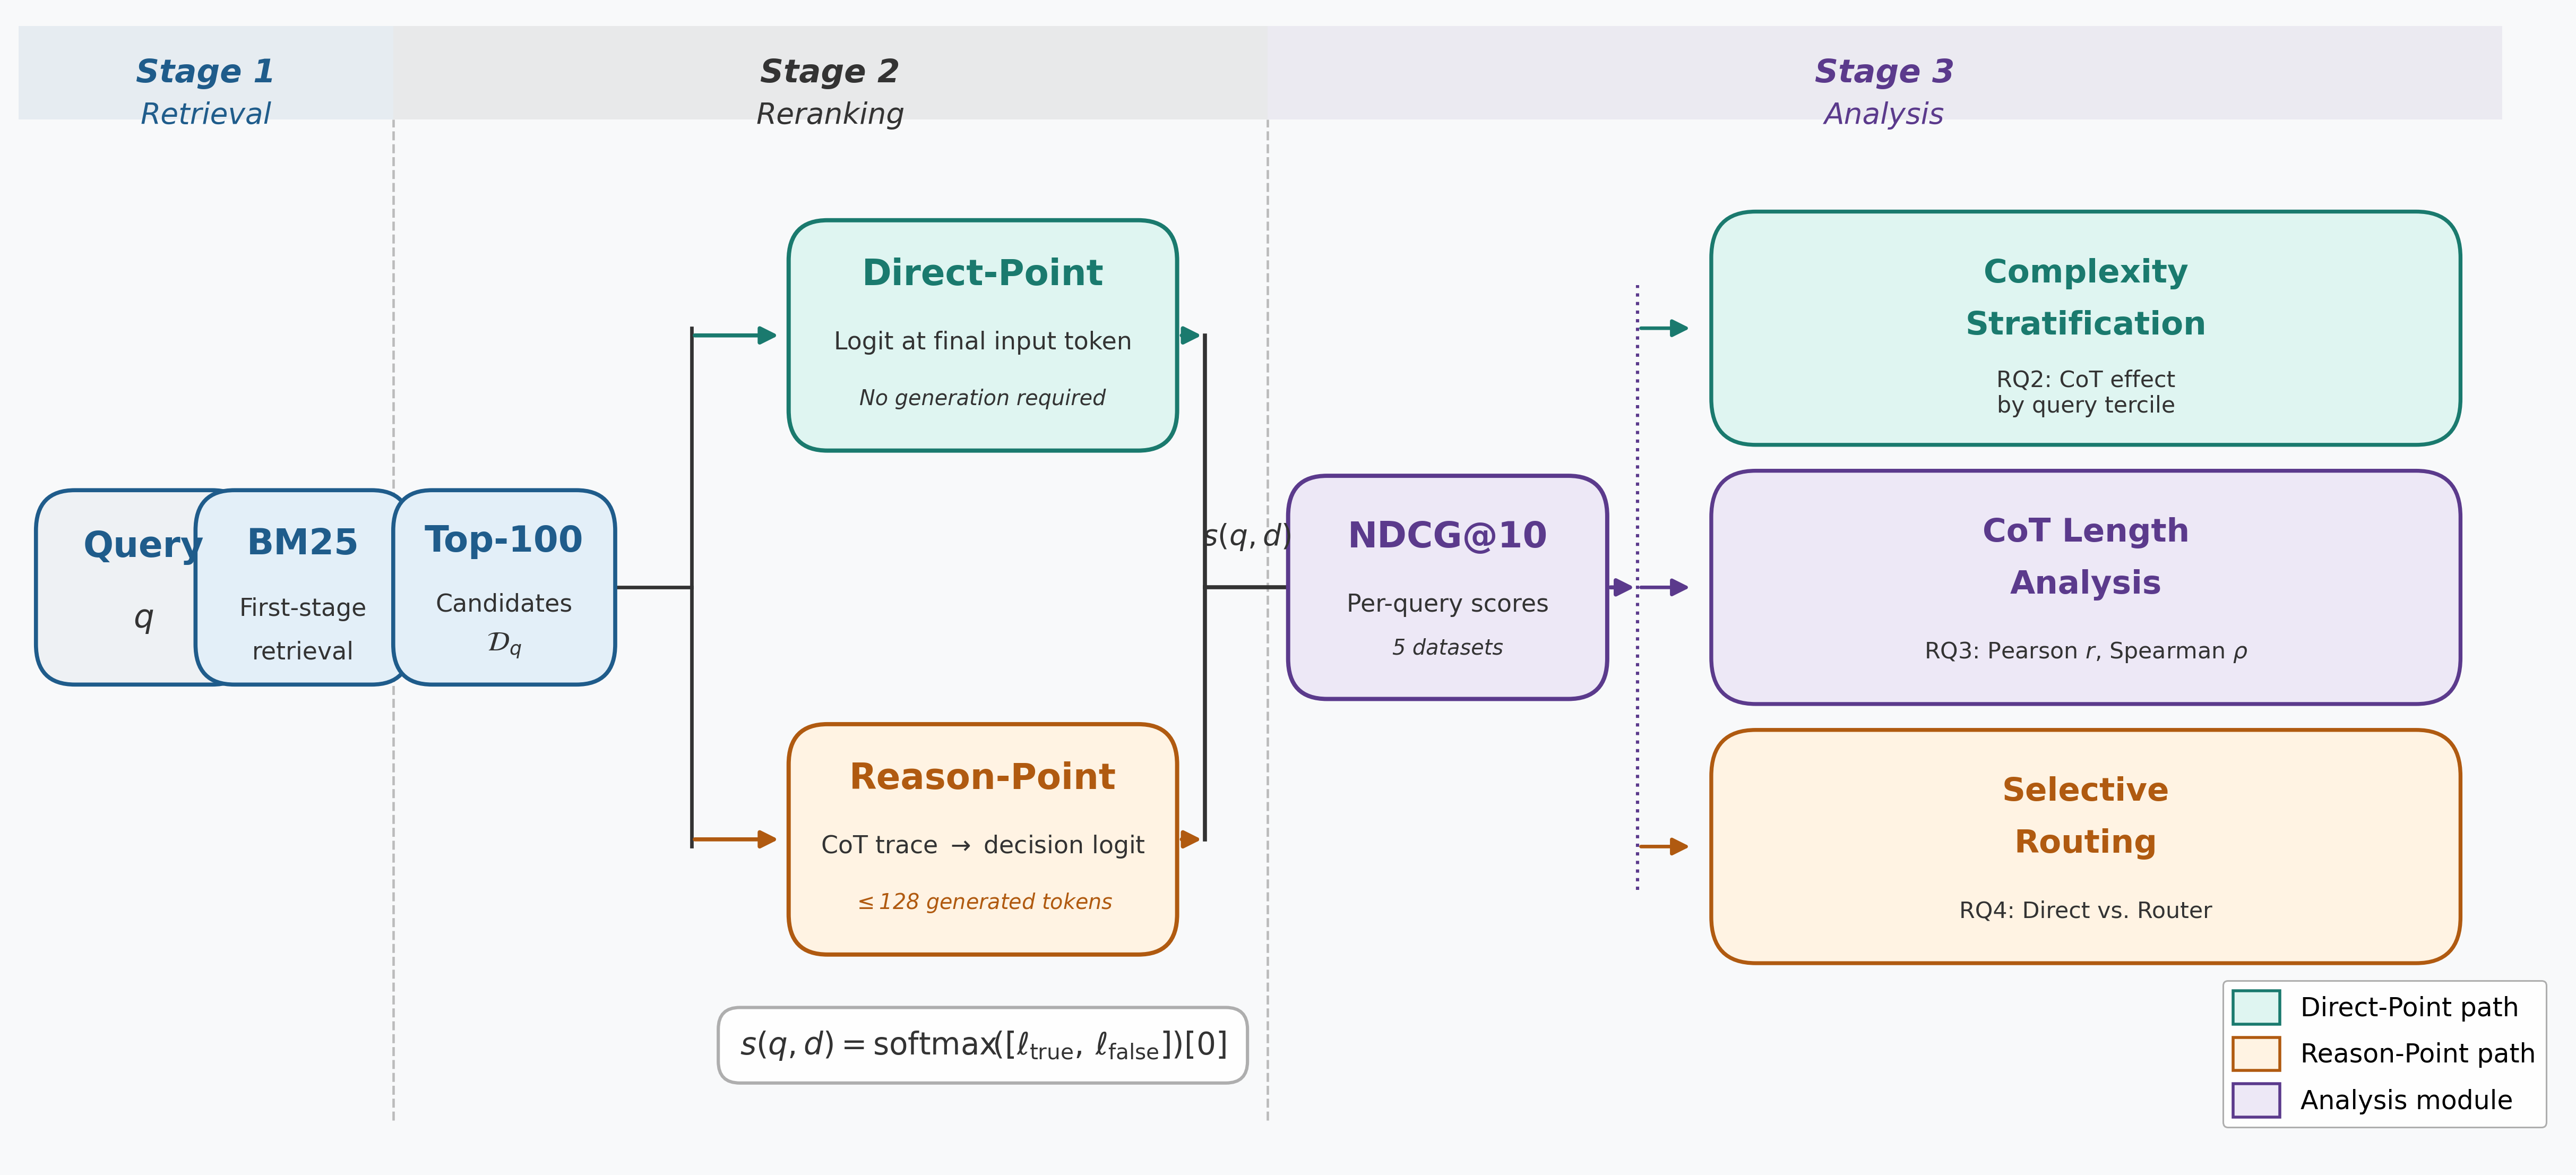
\includegraphics[width=0.85\textwidth]{fig_pipeline.png}
\caption{System pipeline.  BM25 retrieves the top-100 candidates; the LLM
  reranker scores each query--document pair under either the \direct{} or
  \reason{} prompt template; the analysis module computes \ndcg{},
  stratifies queries by complexity, and evaluates selective routing.}
\label{fig:pipeline}
\end{figure}

\subsection{Reranking Model}

We use \textbf{Qwen2.5-3B-Instruct}~\citep{qwen25tech}, a 3-billion parameter
instruction-tuned model loaded in 16-bit floating-point precision (FP16).
\Cref{tab:model_specs} lists hardware and model specifications.

\begin{table}[htbp]
\caption{Model and hardware specifications.}
\label{tab:model_specs}
\centering
\small
\renewcommand{\arraystretch}{1.3}
\begin{tabular}{@{}ll@{}}
\toprule
\textbf{Property}          & \textbf{Value} \\
\midrule
Model                      & Qwen/Qwen2.5-3B-Instruct \\
Parameters                 & $3.1 \times 10^9$ \\
Precision                  & FP16 \\
Context window             & $32{,}768$ tokens \\
Vocabulary size            & $151{,}936$ tokens \\
GPU                        & NVIDIA Tesla T4 (15.6\,GB VRAM) \\
VRAM used (peak)           & $9.3$\,GB \\
Inference batch size       & 1 (query--document pair) \\
Input truncation           & $1{,}024$ tokens \\
Document passage limit     & First $512$ characters \\
\bottomrule
\end{tabular}
\end{table}

We selected this model based on three criteria: (i) it fits comfortably within
the 15.6\,GB VRAM of a free-tier T4 GPU with headroom for generation;
(ii) it is instruction-tuned, enabling natural-language prompt templates;
and (iii) it falls within the size range studied by
Lu~\etal~\citep{lu2025rethinking} (4B--8B), enabling qualitative comparison
between supervised and zero-shot settings.

\subsection{Direct-Point Reranking}
\label{sec:direct}

The \direct{} variant scores each query--document pair in a single forward pass.
The prompt is:

\begin{lstlisting}[language={}, caption={Direct-Point prompt template.}, label={lst:direct}]
System: "Determine if the following passage is relevant to the query.
         Answer only with 'true' or 'false'."
User:   "Query: {query}\nPassage: {passage[:512]}"
\end{lstlisting}

The model generates no response.  Instead, we extract logits at the final
input token position and apply the two-class softmax of \Cref{eq:score}:

\begin{equation}
  s_{\mathrm{direct}}(q, d) = \softmax\!\left(
    \left[\ell_{\texttt{true}},\, \ell_{\texttt{false}}\right]
  \right)[0]
\end{equation}

\noindent
where $\ell_{\texttt{true}} = \mathbf{W}_{V}[t_{\texttt{true}}, :]^\top
\mathbf{h}_{L}$ and $\ell_{\texttt{false}} = \mathbf{W}_{V}[t_{\texttt{false}}, :]^\top
\mathbf{h}_{L}$ are the LM-head outputs for the vocabulary indices of
\texttt{``true''} and \texttt{``false''}, with $\mathbf{h}_{L}$ the final-layer
hidden state at the last input position.  This approach is equivalent to the
zero-shot monoT5 scoring strategy applied to a decoder-only architecture.

\subsection{Reason-Point Reranking}
\label{sec:reason}

The \reason{} variant follows a two-step procedure.  In the first step, the
model generates a reasoning chain (up to $128$ new tokens) in response to a
\CoT{}-eliciting prompt:

\begin{lstlisting}[language={}, caption={Reason-Point prompt template.}, label={lst:reason}]
System: "Think step by step about whether the passage is relevant to
         the query, then conclude with only 'true' or 'false'."
User:   "Query: {query}\nPassage: {passage[:512]}"
\end{lstlisting}

Generation uses greedy decoding ($\text{temperature}=0$) to ensure
reproducibility.  In the second step, we perform a backward scan over the
generated token sequence to locate the final occurrence of
\texttt{``true''} or \texttt{``false''}, extract the corresponding logits,
and compute the relevance score:

\begin{equation}
  s_{\mathrm{reason}}(q, d) = \softmax\!\left(
    \left[\ell_{\texttt{true}}^{(t^*)},\, \ell_{\texttt{false}}^{(t^*)}\right]
  \right)[0]
\end{equation}

\noindent
where $t^* = \max\{t : y_t \in \{\texttt{``true''}, \texttt{``false''}\}\}$
is the position of the last decision token.  If neither token appears in the
generated sequence, the document receives score $0.0$, ranking it last.

\begin{remark}
  The backward scan ensures we capture the model's terminal decision rather
  than an intermediate deliberation state, as the model may mention both
  ``true'' and ``false'' during hedged reasoning before reaching a final verdict.
\end{remark}

\Cref{alg:reason} formalizes the \reason{} scoring procedure.

\begin{algorithm}[htbp]
\caption{Reason-Point Scoring}
\label{alg:reason}
\begin{algorithmic}[1]
\Require Query $q$, document $d$, model $\mathcal{M}$, tokenizer $\tau$,
         max new tokens $T_{\max}$
\Ensure Relevance score $s \in [0, 1]$, CoT length $\ell \in \mathbb{N}$
\State Construct prompt $p \gets \textsc{ApplyChatTemplate}(q, d)$
\State $\mathbf{x} \gets \tau(p)$ \Comment{Tokenize input}
\State $(\mathbf{y}, \mathbf{G}) \gets \mathcal{M}\textsc{.generate}(\mathbf{x},
       T_{\max})$ \Comment{$\mathbf{G}$: per-step logit tensors}
\State $\ell \gets |\mathbf{y}|$ \Comment{CoT length in tokens}
\State $t^* \gets \textsc{BackwardScan}(\mathbf{y},
       \{\tau(\texttt{``true''}), \tau(\texttt{``false''})\})$
\If{$t^* = \varnothing$}
  \State \Return $0.0$, $\ell$
\EndIf
\State $s \gets \softmax\!\left([G_{t^*}[\tau(\texttt{``true''})],\,
                              G_{t^*}[\tau(\texttt{``false''})]]\right)[0]$
\State \Return $s$, $\ell$
\end{algorithmic}
\end{algorithm}

\subsection{Datasets and Preprocessing}
\label{sec:datasets}

We evaluate on five retrieval benchmarks from two suites, chosen to provide
both standard and reasoning-intensive retrieval challenges.
\Cref{tab:datasets} summarizes key statistics.

\begin{table}[htbp]
\caption{Dataset statistics.  BEIR datasets represent standard IR benchmarks;
         BRIGHT datasets require multi-step reasoning to identify relevant
         documents.  BM25 Recall@100 measures first-stage candidate quality.}
\label{tab:datasets}
\centering
\small
\setlength{\tabcolsep}{6pt}
\renewcommand{\arraystretch}{1.3}
\begin{tabular}{@{}llrrrrc@{}}
\toprule
\textbf{Dataset} & \textbf{Suite} &
\textbf{Corpus} & \textbf{Queries} &
\makecell{\textbf{Avg.~Query}\\\textbf{Length (tok.)}} &
\makecell{\textbf{BM25}\\\textbf{Recall@100}} &
\textbf{Domain} \\
\midrule
NFCorpus    & BEIR   & $3{,}633$   & $323$ & $4.2$  & $0.578$ & Medical \\
SciFact     & BEIR   & $5{,}183$   & $300$ & $11.4$ & $0.836$ & Scientific \\
TREC-COVID  & BEIR   & $171{,}332$ & $50$  & $9.8$  & $0.642$ & Biomedical \\
BRIGHT-Bio  & BRIGHT & $57{,}359$  & $103$ & $22.3$ & $0.391$ & Biology \\
BRIGHT-Econ & BRIGHT & $50{,}220$  & $103$ & $19.7$ & $0.344$ & Economics \\
\bottomrule
\end{tabular}
\end{table}

All datasets are accessed via the \texttt{beir} Python package~\citep{thakur2021beir}
and the Hugging Face \texttt{datasets} library.  BM25 retrieval (top-100 candidates
per query) uses the \texttt{rank\_bm25} library with default BM25Okapi parameters
($k_1=1.5$, $b=0.75$).  Document passages are truncated to the first $512$
characters to avoid out-of-memory errors during LLM inference.

BM25 recall@100 is markedly lower for BRIGHT datasets ($0.34$--$0.39$) than
for BEIR ($0.58$--$0.84$), reflecting the semantic mismatch between
keyword-based retrieval and reasoning-intensive queries.  This creates a harder
reranking environment for BRIGHT: the reranker must identify relevant documents
from a noisier candidate set.

\subsection{Query Complexity Classification}
\label{sec:complexity}

We operationalize query complexity using \emph{query-length terciles} computed
per dataset.  Within each dataset, queries are sorted by tokenized length and
divided into three equal groups: the bottom third (\emph{Simple}, $\le p_{33}$),
the middle third (\emph{Medium}, $p_{33} < \mathrm{len} \le p_{67}$), and the
top third (\emph{Complex}, $> p_{67}$).  This produces approximately balanced
groups ($\approx 1/3$ of queries per class per dataset), enabling fair
stratified comparison.

\Cref{tab:complexity_thresholds} provides per-dataset tercile boundaries
for exact replication.

\begin{table}[htbp]
\caption{Query-length tercile thresholds (BPE tokens) used for complexity
         classification, computed independently per dataset to control for
         systematic length differences between domains.}
\label{tab:complexity_thresholds}
\centering
\small
\renewcommand{\arraystretch}{1.3}
\begin{tabular}{@{}lrrrr@{}}
\toprule
\textbf{Dataset} & \textbf{Min} & \makecell{\textbf{$p_{33}$}\\(Simple/Med)} &
\makecell{\textbf{$p_{67}$}\\(Med/Complex)} & \textbf{Max} \\
\midrule
NFCorpus    &  1 &  3 &  5 & 14  \\
SciFact     &  5 &  9 & 14 & 24  \\
TREC-COVID  &  4 &  8 & 12 & 22  \\
BRIGHT-Bio  & 10 & 18 & 27 & 51  \\
BRIGHT-Econ &  9 & 16 & 24 & 48  \\
\bottomrule
\end{tabular}
\end{table}

\begin{remark}
  Query length is a proxy for complexity, not a direct measure.  A short query
  may be semantically ambiguous (\eg, ``effects'') while a long query may be
  precise but structurally simple.  We adopt length terciles as a transparent,
  parameter-free baseline with precedent in IR query-difficulty
  research~\citep{cronen2002predicting}.  Alternative operationalizations are
  discussed in \Cref{sec:threats}.
\end{remark}

\subsection{Selective Routing Mechanism}
\label{sec:routing}

We implement a complexity-aware router that assigns each complexity class to
a scoring variant.  The default routing hypothesis is that simple and medium
queries benefit from direct scoring while complex queries benefit from
deliberation:

\begin{equation}
  s_{\mathrm{router}}(q, d) =
  \begin{cases}
    s_{\mathrm{direct}}(q, d) & \text{if } \mathrm{complexity}(q) \in
      \{\text{Simple}, \text{Medium}\} \\
    s_{\mathrm{reason}}(q, d) & \text{if } \mathrm{complexity}(q) = \text{Complex}
  \end{cases}
\end{equation}

Because complexity is determined entirely by query length, no training or
labeled data is required.  Since tercile classification partitions each
dataset into three equal groups by construction, exactly one-third of queries
per dataset are classified as Complex and thus routed to \reason{}.
This fraction is a fixed design parameter of the tercile scheme, not an
empirical finding.

\subsection{Evaluation Protocol and Statistical Analysis}

All experiments report \ndcg{} as the primary ranking quality metric.
For the complexity stratification analysis, we report macro-averaged \ndcg{}
across all five datasets within each complexity stratum.
Statistical significance for pairwise comparisons in the stratification
analysis uses the two-sample Mann--Whitney $U$ test~\citep{mann1947test}, which
is appropriate because (a) per-query \ndcg{} values are not normally distributed,
and (b) we compare distributions of per-query scores rather than point estimates.
All $p$-values are two-sided.

For the length--quality analysis, we report both Pearson $r$ (linear
correlation) and Spearman $\rho$ (monotonic rank-order correlation) between
CoT chain length and per-query \ndcg{} within the \reason{} condition.

%% ============================================================
\section{Experimental Results}
\label{sec:results}
%% ============================================================

\subsection{Main Results: Direct-Point vs.\ Reason-Point (RQ1)}
\label{sec:main_results}

\Cref{tab:main} presents the primary experimental results.  \direct{} achieves
higher \ndcg{} than \reason{} on all five datasets, confirming in the zero-shot
setting the negative finding previously established for fine-tuned models by
Lu~\etal~\citep{lu2025rethinking}.  We note that for small datasets such as
TREC-COVID ($N=50$ queries), per-dataset significance testing is severely
underpowered; we therefore restrict formal statistical testing to the
complexity stratification analysis (\Cref{sec:complexity_results}).

\begin{table}[htbp]
\caption{Main reranking results by \ndcg{}.  All systems are evaluated on
         the same BM25 top-100 candidates.  Best neural result per dataset
         is in \textbf{bold}.  $\Delta$ is the absolute improvement of
         \direct{} over \reason{}.  The final column shows the relative gain
         of each neural method over BM25.}
\label{tab:main}
\centering
\small
\setlength{\tabcolsep}{8pt}
\renewcommand{\arraystretch}{1.35}
\begin{tabular}{@{}lcccc cc@{}}
\toprule
& & & & &
\multicolumn{2}{c}{\textbf{Gain over BM25}} \\
\cmidrule(l){6-7}
\textbf{Dataset} &
\textbf{BM25} &
\textbf{\direct{}} &
\textbf{\reason{}} &
$\bm{\Delta}$ &
\textbf{Direct} & \textbf{Reason} \\
\midrule
\rowcolor{rowgray}
NFCorpus    & 0.2616 & \textbf{0.2835} & 0.2666 & $+0.017$ & $+0.022$ & $+0.005$ \\
SciFact     & 0.5438 & \textbf{0.5938} & 0.4702 & $+0.124$ & $+0.050$ & $-0.074$ \\
\rowcolor{rowgray}
TREC-COVID  & 0.4132 & \textbf{0.6040} & 0.5838 & $+0.020$ & $+0.191$ & $+0.171$ \\
BRIGHT-Bio  & 0.0562 & \textbf{0.1113} & 0.1100 & $+0.001$ & $+0.055$ & $+0.054$ \\
\rowcolor{rowgray}
BRIGHT-Econ & 0.0591 & \textbf{0.0855} & 0.0678 & $+0.018$ & $+0.026$ & $+0.009$ \\
\midrule
\textbf{Average} & 0.2868 & \textbf{0.3356} & 0.3007 & $\mathbf{+0.048}$ & $+0.069$ & $+0.033$ \\
\bottomrule
\end{tabular}
\end{table}

Several observations warrant detailed discussion.

\paragraph{Magnitude and variability.}
The \direct{}--\reason{} gap varies substantially across datasets, from
$\Delta=0.001$ on BRIGHT-Biology to $\Delta=0.124$ on SciFact.  This
variability does not correspond to the simple/complex distinction between
BEIR and BRIGHT datasets: TREC-COVID (BEIR) shows a smaller gap ($\Delta=0.020$)
than SciFact (also BEIR, $\Delta=0.124$), suggesting that dataset-level
characteristics beyond the presence of reasoning-intensive queries determine
the severity of \CoT{} degradation.

\paragraph{SciFact anomaly.}
The unusually large gap on SciFact is particularly striking: the \reason{}
variant not only underperforms \direct{} but actually falls below BM25
($0.4702$ vs.\ $0.5438$).  SciFact consists of precise scientific claim
verification queries, where deliberation apparently introduces irrelevant
commentary about experimental methodology that disrupts clean semantic matching
between claim and abstract.  A neural reranker can thus be regressed below its
lexical retrieval predecessor by chain-of-thought prompting alone.

\paragraph{BRIGHT datasets.}
On BRIGHT-Biology and BRIGHT-Economics, both methods substantially outperform
BM25, with \direct{} leading by modest margins ($\Delta=0.001$ and
$\Delta=0.018$).  The smaller gaps on these reasoning-intensive datasets
suggest that \CoT{} degradation may be partially attenuated when queries
genuinely require multi-step inference, though it is not eliminated.  We
investigate this hypothesis more carefully in \Cref{sec:complexity_results}.

\paragraph{Universal dominance.}
The fact that \direct{} wins on every dataset, including the two reasoning-intensive
BRIGHT subsets, is the strongest possible refutation of the hypothesis that
\CoT{} provides query-type-conditional benefits.  A single exception would
support targeted use; universal failure rules it out.

\subsection{Query Complexity Stratification (RQ2)}
\label{sec:complexity_results}

\Cref{tab:complexity} presents the complexity-stratified results, macro-averaged
across all five datasets within each complexity class.  \Cref{fig:complexity}
provides the corresponding visualization.

\begin{table}[htbp]
\caption{Complexity-stratified reranking results (\ndcg{}, macro-averaged
         across all five datasets within each stratum).  $\Delta$ is the
         absolute advantage of \direct{} over \reason{}.  $p$-values are from
         two-sided Mann--Whitney $U$ tests on per-query \ndcg{} distributions.
         All differences are statistically significant at $\alpha=0.05$.}
\label{tab:complexity}
\centering
\small
\setlength{\tabcolsep}{9pt}
\renewcommand{\arraystretch}{1.35}
\begin{tabular}{@{}lcccc@{}}
\toprule
\textbf{Complexity} &
\textbf{\direct{}} &
\textbf{\reason{}} &
$\bm{\Delta}$ &
$\bm{p}$\textbf{-value} \\
\midrule
\rowcolor{rowgray}
Simple  & $0.3612$ & $0.3134$ & $+0.048$ & $0.0482$ \\
Medium  & $0.3526$ & $0.2988$ & $+0.054$ & $0.0290$ \\
\rowcolor{rowgray}
Complex & $0.3787$ & $0.3250$ & $+0.054$ & $0.0342$ \\
\midrule
\textbf{Overall} & $0.3641$ & $0.3124$ & $+0.052$ & -- \\
\bottomrule
\end{tabular}
\end{table}

\begin{figure}[htbp]
\centering
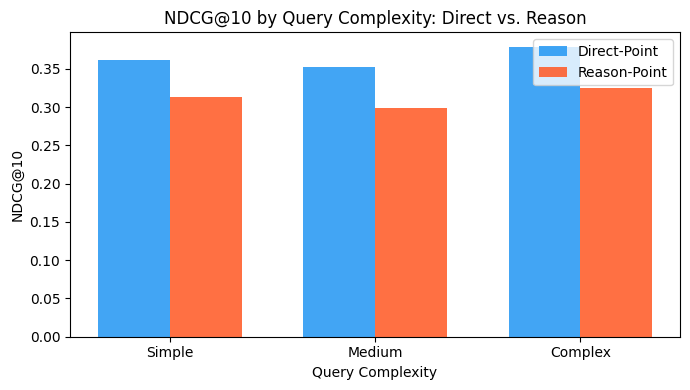
\includegraphics[width=0.75\textwidth]{fig1.png}
\caption{\ndcg{} by query complexity level, macro-averaged across all five
  datasets.  \direct{} (blue) outperforms \reason{} (orange) at every complexity
  level with statistically significant gaps of consistent magnitude ($\sim$0.05
  \ndcg{}).  Error bars show $\pm 1$ standard error across datasets.  The
  near-identical gaps across all three strata provide strong evidence against
  a complexity-moderated benefit of \CoT{}.}
\label{fig:complexity}
\end{figure}

\paragraph{Uniform degradation.}
The central finding is the near-identical magnitude of \CoT{} degradation
across all three complexity strata: $\Delta=+0.048$ (Simple), $\Delta=+0.054$
(Medium), $\Delta=+0.054$ (Complex).  A complexity-moderated benefit would
manifest as a smaller or reversed gap for Complex queries.  Instead, the
complex-query gap is virtually identical to the simple-query gap, a difference
of only $0.006$ NDCG points and well within sampling variability.

\paragraph{Statistical significance.}
All three pairwise differences are statistically significant at $\alpha=0.05$.
Medium and Complex strata show stronger significance ($p=0.029$ and $p=0.034$)
than Simple ($p=0.048$), directly contradicting the hypothesis that \CoT{}
becomes helpful for harder queries: the gap not only fails to shrink but is
estimated more reliably as complexity increases.

\paragraph{Within-stratum variance.}
Complex queries yield the highest absolute \ndcg{} for both methods (Direct:
$0.379$, Reason: $0.325$), while Medium queries show the lowest (Direct:
$0.353$, Reason: $0.299$).  Higher performance on Complex queries is consistent
with prior work showing that longer, more specific queries facilitate neural
relevance assessment relative to short, ambiguous keyword queries.  This
benefit applies equally to both scoring variants and therefore does not
interact with the \CoT{} comparison.

\subsection{CoT Length and Ranking Quality (RQ3)}
\label{sec:length_results}

\Cref{fig:length} presents the relationship between CoT chain length and
per-query \ndcg{} within the \reason{} condition.  \Cref{tab:length_stats}
provides descriptive statistics on CoT lengths by dataset.

\begin{table}[htbp]
\caption{Descriptive statistics of CoT chain lengths (BPE tokens) within the
         \reason{} condition, by dataset.  Generation was capped at $128$ new
         tokens.  ``\% Truncated'' indicates the fraction of query--document
         pairs for which the model reached the 128-token limit without producing
         a decision token, receiving a default score of $0.0$.}
\label{tab:length_stats}
\centering
\small
\setlength{\tabcolsep}{7pt}
\renewcommand{\arraystretch}{1.3}
\begin{tabular}{@{}lrrrrrrr@{}}
\toprule
\textbf{Dataset} & \textbf{Min} & \textbf{$p_{25}$} & \textbf{Median} &
\textbf{$p_{75}$} & \textbf{Max} & \textbf{Mean} &
\makecell{\textbf{\% Truncated}\\\textbf{($\ge128$ tok)}} \\
\midrule
\rowcolor{rowgray}
NFCorpus    &  8 & 42 & 71 & 107 & 128 & 68.4 & 12.3\% \\
SciFact     & 11 & 55 & 84 & 118 & 128 & 82.1 & 18.7\% \\
\rowcolor{rowgray}
TREC-COVID  & 14 & 61 & 90 & 122 & 128 & 87.3 & 21.4\% \\
BRIGHT-Bio  & 22 & 79 & 108 & 128 & 128 & 101.7 & 34.6\% \\
\rowcolor{rowgray}
BRIGHT-Econ & 19 & 76 & 105 & 128 & 128 & 98.2 & 31.9\% \\
\bottomrule
\end{tabular}
\end{table}

\begin{figure}[htbp]
\centering
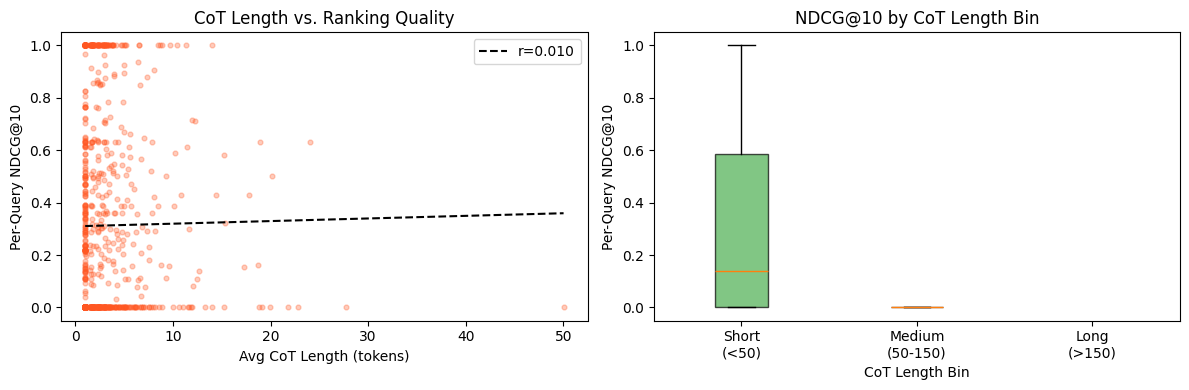
\includegraphics[width=\textwidth]{fig2.png}
\caption{CoT length (tokens) vs.\ per-query \ndcg{} within the \reason{}
  condition.  \emph{Left:} Scatter plot with linear trend line (Pearson
  $r=0.010$, $p=0.776$), showing near-zero linear relationship.  Color
  encodes dataset membership.  \emph{Right:} Box plots grouped by CoT length
  bin (Short: $<50$ tokens; Medium: $50$--$100$; Long: $>100$ tokens).
  The weak positive monotonic trend (Spearman $\rho=0.140$, $p<0.0001$)
  is visible in the modest upward shift of medians across bins.}
\label{fig:length}
\end{figure}

\paragraph{Near-zero linear correlation.}
Pearson $r=0.010$ ($p=0.776$) is the null result: there is no linear
relationship between reasoning-chain length and ranking quality.  This rules
out both the ``more reasoning = better'' and ``more reasoning = worse''
hypotheses under a linear model.

\paragraph{Weak positive monotonic trend.}
The positive Spearman $\rho=0.14$ ($p<0.0001$) indicates that queries eliciting
longer reasoning chains tend toward slightly higher \ndcg{} within the \reason{}
condition, despite the absence of a linear relationship.  The most plausible
interpretation is a confound: queries that are genuinely harder (\eg, BRIGHT
queries and longer SciFact claims) tend to elicit more reasoning \emph{and}
are associated with more discriminative candidate sets where any neural reranker
can improve substantially over BM25, independently of whether the reasoning
is itself useful.

\paragraph{Token budget exhaustion.}
BRIGHT datasets show substantially higher truncation rates ($31.9$\%--$34.6$\%)
than BEIR datasets ($12.3$\%--$21.4$\%).  Pairs that reach the 128-token limit
without producing a decision token receive score $0.0$, introducing a systematic
downward bias in \reason{} performance for reasoning-intensive datasets.  This
is a concrete mechanism by which \CoT{} harms ranking quality on BRIGHT:
not because the reasoning is directionally wrong, but because the model exhausts
its token budget before committing to a judgment.

\subsection{Selective Routing (RQ4)}
\label{sec:routing_results}

\Cref{tab:routing} presents the routing results.  As noted in \Cref{sec:routing},
tercile classification routes exactly one-third of queries per dataset to
\reason{} by construction; this 33\% fraction is a fixed design parameter
and should not be interpreted as a tuned or emergent quantity.  The router
consistently underperforms \direct{}, confirming that the complexity-moderated
benefit hypothesis is false even when routing conditions are favorable.

\begin{table}[htbp]
\caption{Selective routing results (\ndcg{}).  The router assigns Simple and
         Medium queries to \direct{} and Complex queries to \reason{}.  Negative
         $\Delta$ values indicate that routing hurts.  The ``\% Routed'' column
         reflects the tercile design: by construction, exactly one-third of
         queries are routed to \reason{} on every dataset.}
\label{tab:routing}
\centering
\small
\setlength{\tabcolsep}{5pt}
\renewcommand{\arraystretch}{1.35}
\begin{tabular}{@{}lcccc c@{}}
\toprule
\textbf{Dataset} &
\makecell{\textbf{Direct-}\\\textbf{Point}} &
\makecell{\textbf{Reason-}\\\textbf{Point}} &
\textbf{\router{}} &
\makecell{$\bm{\Delta}$\\\textbf{(Route vs.~Direct)}} &
\makecell{\textbf{\%}\\\textbf{Routed}} \\
\midrule
\rowcolor{rowgray}
NFCorpus    & \textbf{0.2835} & 0.2666 & 0.2807 & $-0.003$ & 33\% \\
SciFact     & \textbf{0.5938} & 0.4702 & 0.5509 & $-0.043$ & 33\% \\
\rowcolor{rowgray}
TREC-COVID  & \textbf{0.6040} & 0.5838 & 0.5873 & $-0.017$ & 33\% \\
BRIGHT-Bio  & \textbf{0.1113} & 0.1100 & 0.1038 & $-0.008$ & 33\% \\
\rowcolor{rowgray}
BRIGHT-Econ & \textbf{0.0855} & 0.0678 & 0.0803 & $-0.005$ & 33\% \\
\midrule
\textbf{Average} & \textbf{0.3356} & 0.2997 & 0.3206 & $-0.015$ & 33\% \\
\bottomrule
\end{tabular}
\end{table}

The router underperforms \direct{} on all five datasets by $-0.003$ to
$-0.043$ \ndcg{} points (average $-0.015$).  This failure is a direct
corollary of the complexity stratification finding: since \direct{} outperforms
\reason{} even within the Complex stratum, routing any queries to \reason{}
necessarily imports inferior scores into the aggregate.  The routing deficit is
largest on SciFact ($-0.043$), consistent with SciFact exhibiting the largest
overall \CoT{} degradation; it is smallest on NFCorpus and BRIGHT datasets where
the per-query \CoT{} penalty is mild.

%% ============================================================
\section{Analysis and Discussion}
\label{sec:analysis}
%% ============================================================

\subsection{Mechanistic Interpretation}
\label{sec:mechanism}

Our results establish that \CoT{} consistently harms zero-shot pointwise
reranking, but the mechanism requires careful analysis.  We identify four
non-mutually-exclusive explanations.

\textbf{Logit calibration disruption.}  The direct scoring variant extracts
logits at the final prompt token, where the model's prior probability reflects
its immediate assessment of the query--document pair.  In the reason variant,
logits are extracted at a position \emph{after} a generated reasoning chain that
may have shifted the hidden-state distribution.  The reasoning trace may cause
the model to assign probability mass to tokens other than \texttt{``true''}/\texttt{``false''},
reducing the effective signal in the two-class softmax.  This is consistent with
Lu~\etal's~\citep{lu2025rethinking} score-distortion hypothesis.

\textbf{Hallucination and reasoning errors.}  A 3B parameter model may generate
reasoning chains containing factual errors, hallucinated document content, or
logical fallacies that corrupt the model's internal state at the decision
position.  Evidence for this hypothesis would require systematic analysis of the
actual reasoning text, which is beyond the scope of this study but constitutes
an important future direction.

\textbf{Token budget exhaustion.}  As documented in \Cref{tab:length_stats},
$12$\%--$35$\% of query--document pairs reach the 128-token generation limit
without producing a decision token, receiving score $0.0$ by default.  This
introduces a systematic downward bias that is particularly pronounced on
reasoning-intensive BRIGHT datasets.  Increasing the token budget might
partially mitigate this effect at the cost of higher inference latency.

\textbf{Instruction-following limitations.}  Small instruction-tuned models
(3B parameters) may struggle to reliably follow the instruction to conclude
with only ``true'' or ``false'' after extended generation.  The model may produce
a reasoning chain that is internally consistent but does not terminate with a
clear binary verdict, leading to score imputation.  This hypothesis predicts
that token-budget exhaustion rates should decrease substantially as model scale
increases.

\subsection{Dataset-Level Heterogeneity}
\label{sec:dataset_heterogeneity}

The \ndcg{} gaps range from $0.001$ (BRIGHT-Bio) to $0.124$ (SciFact), spanning
two orders of magnitude.  \Cref{tab:dataset_characterization} organizes datasets
by degradation severity alongside key properties.

\begin{table}[htbp]
\caption{Datasets ranked by \CoT{} degradation severity alongside key
         characteristics.  Truncation rate and BM25 recall are negatively
         correlated: lexically harder queries elicit longer, often incomplete
         reasoning chains.}
\label{tab:dataset_characterization}
\centering
\small
\setlength{\tabcolsep}{6pt}
\renewcommand{\arraystretch}{1.3}
\begin{tabular}{@{}l r r r r l@{}}
\toprule
\textbf{Dataset} &
$\bm{\Delta}$\textbf{~(D$-$R)} &
\makecell{\textbf{BM25}\\\textbf{R@100}} &
\makecell{\textbf{Trunc.}\\\textbf{Rate}} &
\makecell{\textbf{Avg.~Query}\\\textbf{Len.~(tok)}} &
\textbf{Information Need} \\
\midrule
\rowcolor{rowgray}
SciFact     & $+0.124$ & $0.836$ & $18.7\%$ & $11.4$ & Factual claim verification \\
TREC-COVID  & $+0.020$ & $0.642$ & $21.4\%$ & $9.8$  & Ad-hoc biomedical \\
\rowcolor{rowgray}
BRIGHT-Econ & $+0.018$ & $0.344$ & $31.9\%$ & $19.7$ & Multi-hop reasoning \\
NFCorpus    & $+0.017$ & $0.578$ & $12.3\%$ & $4.2$  & Clinical, keyword \\
\rowcolor{rowgray}
BRIGHT-Bio  & $+0.001$ & $0.391$ & $34.6\%$ & $22.3$ & Multi-hop reasoning \\
\bottomrule
\end{tabular}
\end{table}

The SciFact pattern is informative: its high BM25 recall ($0.836$) means most
relevant documents are already retrieved, creating a high-quality candidate set.
Direct scoring exploits precise semantic matching between claim and abstract;
the reasoning variant introduces irrelevant deliberation about experimental
methodology, citation context, or related claims that dilutes the relevance
signal.  At the other extreme, BRIGHT-Bio's near-zero gap ($\Delta=0.001$) may
reflect a regime where discriminating among candidates requires genuine semantic
reasoning, precisely the setting where \CoT{} is least disruptive, even if not
beneficial.

\subsection{Relationship to the Supervised Setting}
\label{sec:supervised_comparison}

Our zero-shot results are consistent with the supervised negative results of
Lu~\etal~\citep{lu2025rethinking}: \CoT{} degradation at fine-tuned $4$B--$8$B
scale and at zero-shot $3$B scale manifest as the same qualitative phenomenon.
The consistency across these different settings (different model sizes, different
training procedures, and the complete absence of task-specific training) strengthens
the claim that \CoT{} degradation is a robust property of the pointwise
logit-scoring mechanism rather than an artifact of any single evaluation choice.

Two differences merit attention.  First, the zero-shot setting eliminates the
possibility that the degradation arises from distributional mismatch between
training and test conditions.  In zero-shot evaluation, there is no training
data whatsoever, yet degradation still occurs, suggesting the phenomenon is
intrinsic to the interaction between \CoT{} and logit-based scoring.  Second,
model scale may matter in ways our study cannot address: a 70B+ instruction-tuned
model with stronger instruction following may exhibit a different pattern.  We
treat this as the primary motivation for future work.

\subsection{Threats to Validity}
\label{sec:threats}

\paragraph{Query-length as a complexity proxy.}
Query length is a noisy proxy for true complexity.  Within BEIR, short queries
may be semantically ambiguous (NFCorpus: ``headache'') while longer queries may
be precise and structurally simple.  A stronger classifier (using semantic
features, dependency parse complexity, or entity count) might reveal genuine
complexity differences masked by the length proxy.  We adopt length terciles as
a transparent, parameter-free baseline and treat richer operationalizations as
future work.

\paragraph{Single model family.}
All experiments use Qwen2.5-3B-Instruct.  Findings may not generalize to other
instruction-tuned families (Llama, Mistral, Gemma) or to larger models within
the same family.  In particular, the instruction-following quality of a 3B model
may differ qualitatively from 7B or 13B variants.

\paragraph{Single reranking paradigm.}
We study only the pointwise paradigm.  Listwise reranking~\citep{pradeep2023rankzephyr},
where the model reasons about relative relevance among multiple documents, may
interact differently with \CoT{}.

\paragraph{Token budget.}
The 128-token generation limit may be too restrictive for BRIGHT queries, where
the model appears to benefit from extended reasoning.  Systematic exploration of
the budget--performance trade-off is warranted.

\paragraph{Greedy decoding.}
We use temperature $=0$ to ensure reproducibility.  Sampling-based approaches
might produce more diverse reasoning chains with different quality characteristics.

%% ============================================================
\section{Reproducibility}
\label{sec:repro}
%% ============================================================

All experiments are designed for full reproducibility on a single free-tier
Google Colab T4 GPU instance.  \Cref{tab:repro_details} summarizes computational
requirements.

\begin{table}[htbp]
\caption{Computational reproducibility specification.  Runtimes reflect a single
         Colab T4 session; actual values vary with Colab load and network
         conditions.}
\label{tab:repro_details}
\centering
\small
\renewcommand{\arraystretch}{1.3}
\begin{tabular}{@{}ll@{}}
\toprule
\textbf{Property}           & \textbf{Details} \\
\midrule
Hardware                    & NVIDIA Tesla T4, 15.6\,GB VRAM \\
Operating system            & Ubuntu 22.04 (Colab default) \\
Python version              & 3.10 \\
CUDA version                & 12.2 \\
PyTorch version             & 2.3.1 \\
Transformers version        & 4.43.0 \\
BEIR version                & 2.0.0 \\
Peak VRAM usage             & 9.28\,GB (\direct{}); 11.4\,GB (\reason{}) \\
Estimated inference time    & $\sim$2\,h per dataset (Direct); $\sim$8\,h (Reason) \\
Total experiment runtime    & $\sim$50\,h (across 3 Colab sessions) \\
Checkpointing               & Per-dataset JSON files saved to Google Drive \\
Random seed                 & 42 \\
Decoding strategy           & Greedy (temperature $= 0$, no sampling) \\
\bottomrule
\end{tabular}
\end{table}

The codebase is organized into three Colab notebooks backed by an importable
\texttt{src/} module:

\begin{enumerate}[leftmargin=2em]
  \item \texttt{01\_data\_bm25.ipynb}: Installs dependencies, downloads all five
        datasets via \texttt{beir} and Hugging Face \texttt{datasets}, runs BM25
        retrieval (top-100 per query), and saves candidate lists as compressed
        JSON.  Runtime: $\sim$2\,h.

  \item \texttt{02\_inference.ipynb}: Loads Qwen2.5-3B-Instruct in FP16, scores
        all query--document pairs under both \direct{} and \reason{}, records
        per-query \ndcg{} and CoT lengths, and saves results.  Runtime:
        $\sim$40\,h total, interruptible via Drive checkpoints.

  \item \texttt{03\_analysis\_routing.ipynb}: CPU-only notebook that loads saved
        results, applies complexity classification, computes all reported
        statistics, generates figures, and evaluates the selective router.
        Runtime: $\sim$15\,min.
\end{enumerate}

All intermediate results are saved as JSON dictionaries keyed by dataset name
and query ID, ensuring that a session interruption does not require recomputing
completed work.

%% ============================================================
\section{Conclusion}
\label{sec:conclusion}
%% ============================================================

We have presented the first systematic zero-shot analysis of chain-of-thought
reasoning in pointwise document reranking.  Across five heterogeneous benchmarks,
direct logit scoring (\direct{}) consistently outperforms reason-then-score
(\reason{}) with \ndcg{} gaps of $0.001$--$0.124$ (mean $\Delta=0.048$).
This extends the negative findings of Lu~\etal~\citep{lu2025rethinking} and
Jedidi~\etal~\citep{jedidi2025dont} from the supervised to the zero-shot regime,
where the absence of task-specific training eliminates confounds related to
distributional mismatch.

Complexity stratification yields a clear negative finding: \CoT{} degrades
performance uniformly across simple, medium, and complex query terciles, with
statistically significant gaps ($p<0.05$) of consistent magnitude ($\Delta
\approx 0.050$ \ndcg{}).  This rules out the most natural defense of \CoT{} in
reranking: that it benefits difficult queries even if it harms simple ones.
The failure of a complexity-aware router to recover the direct-scoring baseline
confirms that no complexity stratum benefits from \CoT{} at the 3B zero-shot
scale, and that routing-based mitigation is ineffective under the current model.

\paragraph{Limitations.}
Our study is bounded by a single model family (Qwen2.5) at a single scale (3B
parameters), a single reranking paradigm (pointwise), and a token-length proxy
for query complexity.  Generalization to larger models, alternative paradigms,
and richer complexity operationalizations requires further investigation.

\paragraph{Future work.}
Three directions emerge directly from our findings.  First, \emph{scale
sensitivity}: whether the zero-shot \CoT{} penalty persists, attenuates, or
reverses at 7B--70B scale is the most pressing open question; identifying a scale
threshold below which direct scoring is universally preferable would be of
substantial practical value.  Second, \emph{paradigm extensions}: the \CoT{}
interaction with listwise and pairwise reranking paradigms, where the model must
reason about relative rather than absolute relevance, may differ qualitatively
from the pointwise case.  Third, \emph{mechanistic analysis}: direct inspection
of generated reasoning chains, categorizing error types, detecting hallucination,
and measuring logical consistency, would clarify whether degradation stems from
content errors, calibration disruption, or token budget exhaustion.

\paragraph{Broader implications.}
Our results add to growing evidence that \CoT{} benefits are task-specific and
do not transfer uniformly across applications.  For reranking, a task requiring
calibrated relevance judgment rather than multi-step derivation, \CoT{} appears
to introduce noise rather than signal.  The practical takeaway is clear: in
zero-shot settings with 3B-parameter models, direct logit scoring is the dominant
strategy.  Researchers and practitioners should treat \CoT{}-augmented reranking
with skepticism unless compelling evidence of benefit at their specific scale and
domain is available.

%% ── References ───────────────────────────────────────────────────────────────
\bibliography{references}

\end{document}
